a. Write out the $5\times5$ matrix $A$ from $(2.43)$ for the boundary value problem $u''(x)=f(x)$ with
$u(0)=u(1)=0$ for $h=0.25$.\\
b. Write out the $5\times5$ inverse matrix $A^{-1}$ explicitly for this problem.\\
c. If $f(x)=x$, determine the discrete approximation to the solution of the boundary value problem on
this grid and sketch this solution and the five Green's functions whose sum gives this solution.

\begin{solution}\renewcommand{\qedsymbol}{}\ \\
    We have that
    
    $$A=16\left(\begin{array}{ccccc} 0.0625 & 0 & 0 & 0 & 0 \\ 1 & -2 & 1 & 0 & 0 \\ 0 & 1 & -2 & 1 & 0
                                  \\ 0 & 0 & 1 & -2 & 1 \\ 0 & 0 & 0 & 0 & 0.0625 \end{array}\right)=
          \left(\begin{array}{ccccc} 1 & 0 & 0 & 0 & 0 \\ 16 & -32 & 16 & 0 & 0 \\ 0 & 16 & -32 & 16 & 0
                                  \\ 0 & 0 & 16 & -32 & 16 \\ 0 & 0 & 0 & 0 & 1 \end{array}\right)$$

    By MATLAB, we have that
    
    $$A^{-1}=\frac{1}{16}\left(\begin{array}{ccccc} 16 & 0 & 0 & 0 & 0
                                                 \\ 12 & -0.75 & -0.5 & -0.25 & 4
                                                 \\ 8 & -0.5 & -1 & -0.5 & 8
                                                 \\ 4 & -0.25 & -0.5 & -0.75 & 12
                                                 \\ 0 & 0 & 0 & 0 & 16
                         \end{array}\right)=
    \left(\begin{array}{ccccc} 1 & 0 & 0 & 0 & 0 
                        \\ \frac34 & -\frac{3}{64} & -\frac{1}{32} & -\frac{1}{64} & \frac14
                        \\ \frac12 & -\frac{1}{32} & -\frac{1}{16} & -\frac{1}{32} & \frac12
                        \\ \frac14 & -\frac{1}{64} & -\frac{1}{32} & -\frac{3}{64} & \frac34
                        \\ 0 & 0 & 0 & 0 & 1 
    \end{array}\right)$$

    \begin{center}
        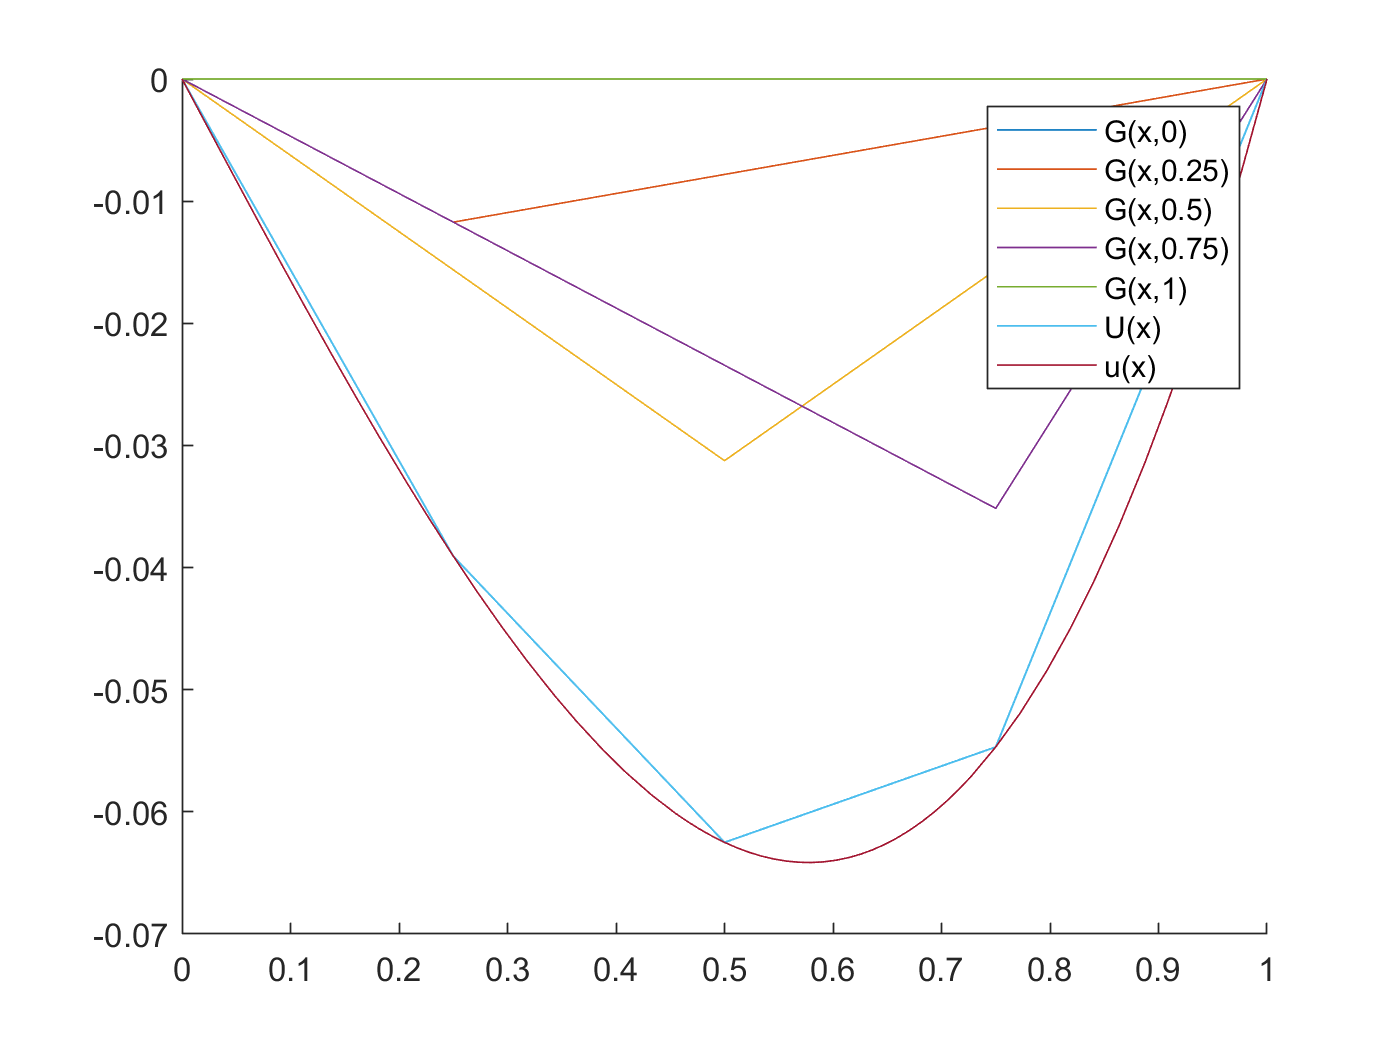
\includegraphics[scale=0.33]{greens.png}
    \end{center}

\end{solution}